\subsection{DSMC法の概要}
希薄流の領域では,連続体近似が破綻し,Navier–Stokes方程式が成立しなくなる.
この場合はBoltzmann方程式を支配方程式として流体解析を行う必要がある.
本研究では,Boltzmann方程式を確率的に解くモンテカルロ直接法~\cite{bird1994molecular} (Direct Simulation Monte Carlo: DSMC) により流星源周りにおける流体場解析を行う.
DSMC法はBoltzmann方程式を解く手法であるが,すべての実在粒子に対して計算を行うのは計算コストが膨大になり現実的ではない.
そこで実在粒子を代表させたDSMC粒子を計算が可能な数配置し,確率的な衝突を介してBoltzmann方程式を解いている.
またDSMC法では,粒子の運動と粒子同士の衝突はカップリングしておらず,それぞれ時間刻み幅の間で別個に計算される.
DSMC法の計算は大きく分けて以下の4つのステップから成る:
\begin{enumerate}
    \item 粒子をそれぞれの持つ速度で時間刻み幅分だけ移動させる.
    \item 移動した粒子の位置からそれぞれの粒子が所属する格子を決定する.
    \item 各格子内部で衝突させる.
    \item 粒子の状態から巨視的な量をサンプリングする.
\end{enumerate}
粒子を配置しそれぞれの運動を追跡するために,計算領域全体は有限の格子に分割される.
初期状態の粒子は乱数を用いてランダムに配置され,位置・速度をそれぞれの粒子に割り当てる.
そして,定常解を得るまで時間刻み幅ごとに反復計算する.
速度・圧力・密度・温度などの巨視的な量は粒子が持つ微視的な量から単純に重み付けし,平均をとることで得る.

\subsection{時間及び空間離散化}
DSMC法でのモデル化において,時間刻み幅内における粒子の運動と粒子間衝突が独立であるという仮定が必要になる.
従って,各粒子はそれぞれの速度を持って時間刻み幅分だけ等速に移動し,その後適当な衝突が行われる.
このような粒子の移動と粒子間衝突を交互に反復することで流れは物理的に現実的な方法で発達する.
粒子の運動と粒子間衝突が独立であるという仮定は,時間刻み幅を平均自由時間よりも短く取ることで成り立つ~\cite{bird1994molecular}.

粒子の適切な衝突相手を選択し,巨視的な量を定義するために計算領域は格子に分割され,空間解像度を上げるほど衝突の距離が短くなるためより多くの粒子が必要になる.
また,DSMC法の計算コスト・計算時間はDSMC粒子数に比例するため,特に低Knudsen数流れの計算では,計算コストと空間解像度のトレードオフを考慮する必要がある.

\subsection{巨視的な量のサンプリング}
DSMC法では粒子の位置・速度が各時間ステップについて計算され,それらの値を用いて密度・圧力・温度などの流れ場の巨視的な量をサンプリングすることができる.
従って,DSMC法も連続流と同様の物理量によって結果を議論することが可能である.

巨視的な量は閉じた格子内に存在する粒子の情報に基づいている必要がある.
数密度が$n$の体積$V$内には実在粒子が$N_r$存在しているとした時,この$N_r$は平均が$nV$で標準偏差が$\sqrt{nV}$のポアソン分布$P$に従い,次の式で表される.
\begin{equation}
    P(N_r) = \dfrac{(nV)^{N_r}}{N_r !}e^{-(nV)}.
\end{equation}
また,統計的に正規化された分散は平均値と標準偏差の比で定義される変動係数$CV$であり,
\begin{equation}
\label{eq:dsmc1.4}
    CV(N_r) = \dfrac{\sqrt{Var(N_r)}}{E(N_r)} = \dfrac{1}{\sqrt{nV}},
\end{equation}
である.
体積$V$内のサンプル粒子数を$N$は,
次式で示される平均値と分散が$nV/F_N$に等しいポアソン分布$P$に従う.
\begin{equation}
    P(N) = \dfrac{\left(nV/F_N\right)^N}{N!} e^{-(nV/F_N)}.
\end{equation}
ここで,$F_N$は1サンプル粒子によって表される実在粒子数であり,その変動係数は以下で表される.
\begin{equation}
\label{eq:dsmc1.6}
    CV(N) = \sqrt{\dfrac{F_N}{nV}}.
\end{equation}
式~(\ref{eq:dsmc1.4})および式~(\ref{eq:dsmc1.6})から,
DSMC法では実在気体の統計的変動が係数$\sqrt{F_N}$で増幅され,
$F_N$は$10^{10}$--$10^{12}$に収まることが分かる.
平均分子間隔$\delta$を使用すると,$nV$は$V/\delta^3$と表せる.
従って,散乱のレベルを妥当なレベルに制限するには,
巨視的な量の瞬時値をサンプリングするセルの大きさが
以下の条件を満たす必要がある.
\begin{equation}
    V^{1/3} \gg (F_N)^{1/3}\delta.
    \label{eq:dsmc1.7}
\end{equation}
さらに,流れ場の解像度を確保するために,
セルの大きさは巨視的勾配のスケール長より小さくする必要がある.
通常,DSMC法の実際のアプリケーションでは,散乱条件に反しない限りは不可能である.
しかし,式~(\ref{eq:dsmc1.7})は瞬間的な平均に対してのみ満たす必要があるため,代替の平均化手法によって達成することが可能になる.

1つの平均化手法は時間平均である.
特定の時間間隔でセル内の巨視的な量を平均化し,定常流を記述する.
2つ目の方法としては,アンサンブル平均である.
同様の条件で複数ケース計算して平均化することで,
非定常流の巨視的な量を確立できる.
これらの手法によって,実質的に全ての流れ場を記述できる.
しかし,両者は確率的であるため,変動の影響をうける.
標準偏差は,サンプルサイズの平方根に反比例するため,
時間平均のサンプリング間隔またはアンサンブル平均の繰り返し数をそれぞれ増やすことで,
任意のレベルまで減らすことが可能である.


\subsection{衝突サンプリング}

衝突を正確にモデル化するために,体積$V_c$のセル内部にある実在気体の粒子数密度$n$の場合を考える.
このセルには$nV_c$個の実在粒子が存在し,平均サンプル粒子数は$\overline{N} = nV_c/F_N$である.
実際のサンプル粒子数は確率変数であり$N$と表す.
運動論によると,このセル内の時間刻み幅$\Delta t$における衝突の総数$N_T$は次式による.
\begin{equation}
    N_T = \dfrac{1}{2}Nv\Delta t = \dfrac{1}{2}Nn\overline{\sigma_Tc_r}\Delta t.
    \label{eq:dsmc1.8}
\end{equation}
ただし,$v = n\overline{\sigma_Tc_r}$である.

セル内の衝突のランダムサンプリングの手法は様々提案されているが,
ここでは一般に広く用いられているno time counter method: NTC法~\cite{gallis2008accuracy}について述べる.

NTC法では,時間刻み幅$\Delta t$で2つの分子間で衝突が発生する確率は,
セル体積に対する相対速度$c_r$での総衝突断面積$F_N\sigma_T$として計算される.
\begin{equation}
    P = \dfrac{F_N\sigma_Tc_r\Delta t}{V_c}.
    \label{eq:dsmc1.9}
\end{equation}
1つのサンプリング確率は,$N(N-1)/2$全ての潜在的なペアについて計算し,
各衝突を対応する発生確率で選択して与える.
ただし通常,$P$は非常に小さく,計算時間はセル内の分子数の2乗に比例するため,
この直接法の効率は低くなる.
したがって,NTC法では,考えられる全ての衝突ペアの一部のみを考慮し,
それらの確率は式~(\ref{eq:dsmc1.9})をこの部分で割ることで増加する.
最大の効率を達成するために,最大確率が1に等しくなるように次式で表される比が選択される.
\begin{equation}
    P_\mathrm{max} = \dfrac{F_N(\sigma_Tc_r)_\mathrm{max}\Delta t}{V_c}.
    \label{eq:dsmc1.10}
\end{equation}
最初に衝突断面積と相対速度の積の最大値である$(\sigma_Tc_r)_\mathrm{max}$を十分大きく選択でき,
シミュレーション中により高い値に更新される.
時間刻み幅での衝突ペアの数は,式~(\ref{eq:dsmc1.10})に$N(N-1)/2$をかけることで得られる.
ただし,$N$は統計的な変動を受けるため,$N(N-1)$を瞬時値またはアンサンブル平均値$N\overline{N}$で置き換えることが推奨される.
また,NTC法の時間刻み幅ごとの衝突とみなされる粒子ペアの数は,
\begin{equation}
    \dfrac{1}{2}\dfrac{N\overline{N}F_N(\sigma_Nc_r)_\mathrm{max}\Delta t}{V_c},
\end{equation}
であり,次式の確率によって選択される.
\begin{equation}
    P = \dfrac{\sigma_Tc_r}{(\sigma_Tc_r)_\mathrm{max}}.
\end{equation}
時間刻み幅ごとに実行される衝突の数は,$P_\mathrm{max}$の正確な値の影響を受けずに,次式に従う.
\begin{equation}
    N_{T,\mathrm{NTC}} = \dfrac{1}{2}\dfrac{N\overline{N}F_N\overline{\sigma_Tc_r\Delta t}}{V_c}
    = \dfrac{1}{2}Nn\overline{\sigma_Tc_r\Delta t}.
\end{equation}
この数は,式~(\ref{eq:dsmc1.8})で得られた理論値と一致し,この手順によって$N$で線形の計算時間が得られる~\cite{bird1994molecular}.



\subsection{希薄流となる条件}
希薄流となる条件は一般的にKnudsen数$Kn$によって定義される.Knudsen数は代表長さと平均自由行程の比で,以下の式で定義される.
\begin{equation}
    Kn = \dfrac{\lambda}{L}.
\end{equation}
ここで,$\lambda$は平均自由行程,$L$は流れの代表長さであり,本研究のように球体周りの場合は球体直径を一般的に用いる.
平均自由行程は仮定によって様々な定義がされるが,本研究ではBird~\cite{bird1994molecular}による以下の式を用いる.
\begin{equation}
    \lambda = \dfrac{1}{\sqrt{2}\pi {d_\mathrm{ref}}^2n\left(T_\mathrm{ref}/T\right)^{\omega - 1/2}}.
\end{equation}
ここで,$d_\mathrm{ref}$は分子直径,$n$は分子数密度,$T_\mathrm{ref}$は地表での大気温度,$T$は大気温度である.また,$\omega$は粘性係数$\mu$と温度$T$を関係付ける係数で,$\mu \propto T^\omega$という形で定義される.

表~\ref{tab:kn-category}に示すのは,Knudsen数によって特徴付けられる,流れの分類である.
$Kn$が0.01より小さいときは流れは連続流とみなすことができ,Navier–Stokes解析が可能になる.
また,$Kn$が10より大きい際は,流れは自由分子流であるとみなすことができ,自由分子流すなわち衝突を考慮しない分子流れの解析が可能になる.
その中間の希薄度の場合,遷移流となり,この領域に関して一般にDSMC法が有効である.
\begin{table}[H]
    \centering
    \caption{Knudsen数による流れの分類}
    \begin{tabular}{c|ccc}
        \hline\hline
        $Kn$ & $Kn < 0.01$ & $0.01 < Kn < 10$ & $ 10 < Kn $ \\ \hline
        流れの分類 & 連続流領域 & 遷移流領域 & 自由分子流領域 \\
        \hline\hline
    \end{tabular}
    \label{tab:kn-category}
\end{table}

\subsection{2体弾性衝突}
粒子の運動を計算するためには,粒子同士の衝突に対する物理モデルが必要である.
希薄流では,3体以上同士の衝突は無視できるほどに稀であるため,DSMC法においては2体衝突のみが考慮される.
ここで考慮する弾性衝突とは,並進エネルギーと内部エネルギーの交換が衝突によって行われないことを意味する.


\subsection{モーメントとエネルギー交換}
質量が$m_1,\ m_2$で,衝突前の速度が$c_1,\ c_2$である2体衝突において衝突後の速度$c_1^*,\ c_2^*$を求めることを考える.
$c_r = c_1 - c_2$を相対速度として,2粒子の重心速度を$c_m$とする.
この時,1次モーメントとエネルギー保存により次が成り立つ~\cite{bird1994molecular}.
\begin{align}
    c_1^* &= c_m + \dfrac{m_2}{m_1 + m_2}c_r^* , \\
    c_2^* &= c_m - \dfrac{m_2}{m_1 + m_2}c_r^* .
\end{align}
相対速度の大きさは衝突によって変化せず,重心は衝突に影響されないので,
相対速度ベクトルの向きの計算は衝突前後の速度変化によって計算される.
また,換算質量$m_r$は以下のように示される.
\begin{equation}
    m_r = \dfrac{m_1 * m_2}{m_1 + m_2}.
\end{equation}
分子間衝突は,多くの場合,分子間力の強い相互作用によって行われる.
分子間力の場は球対称と仮定されることが多く,引力・斥力を持つ.
すなわち,無限大の距離では力が0となり,距離に反比例して強く引きつけられる.
また,衝突の力学は図~\ref{fig:bird1}に示すように,古典的な2体問題として扱われる.

\begin{figure}
    \centering
    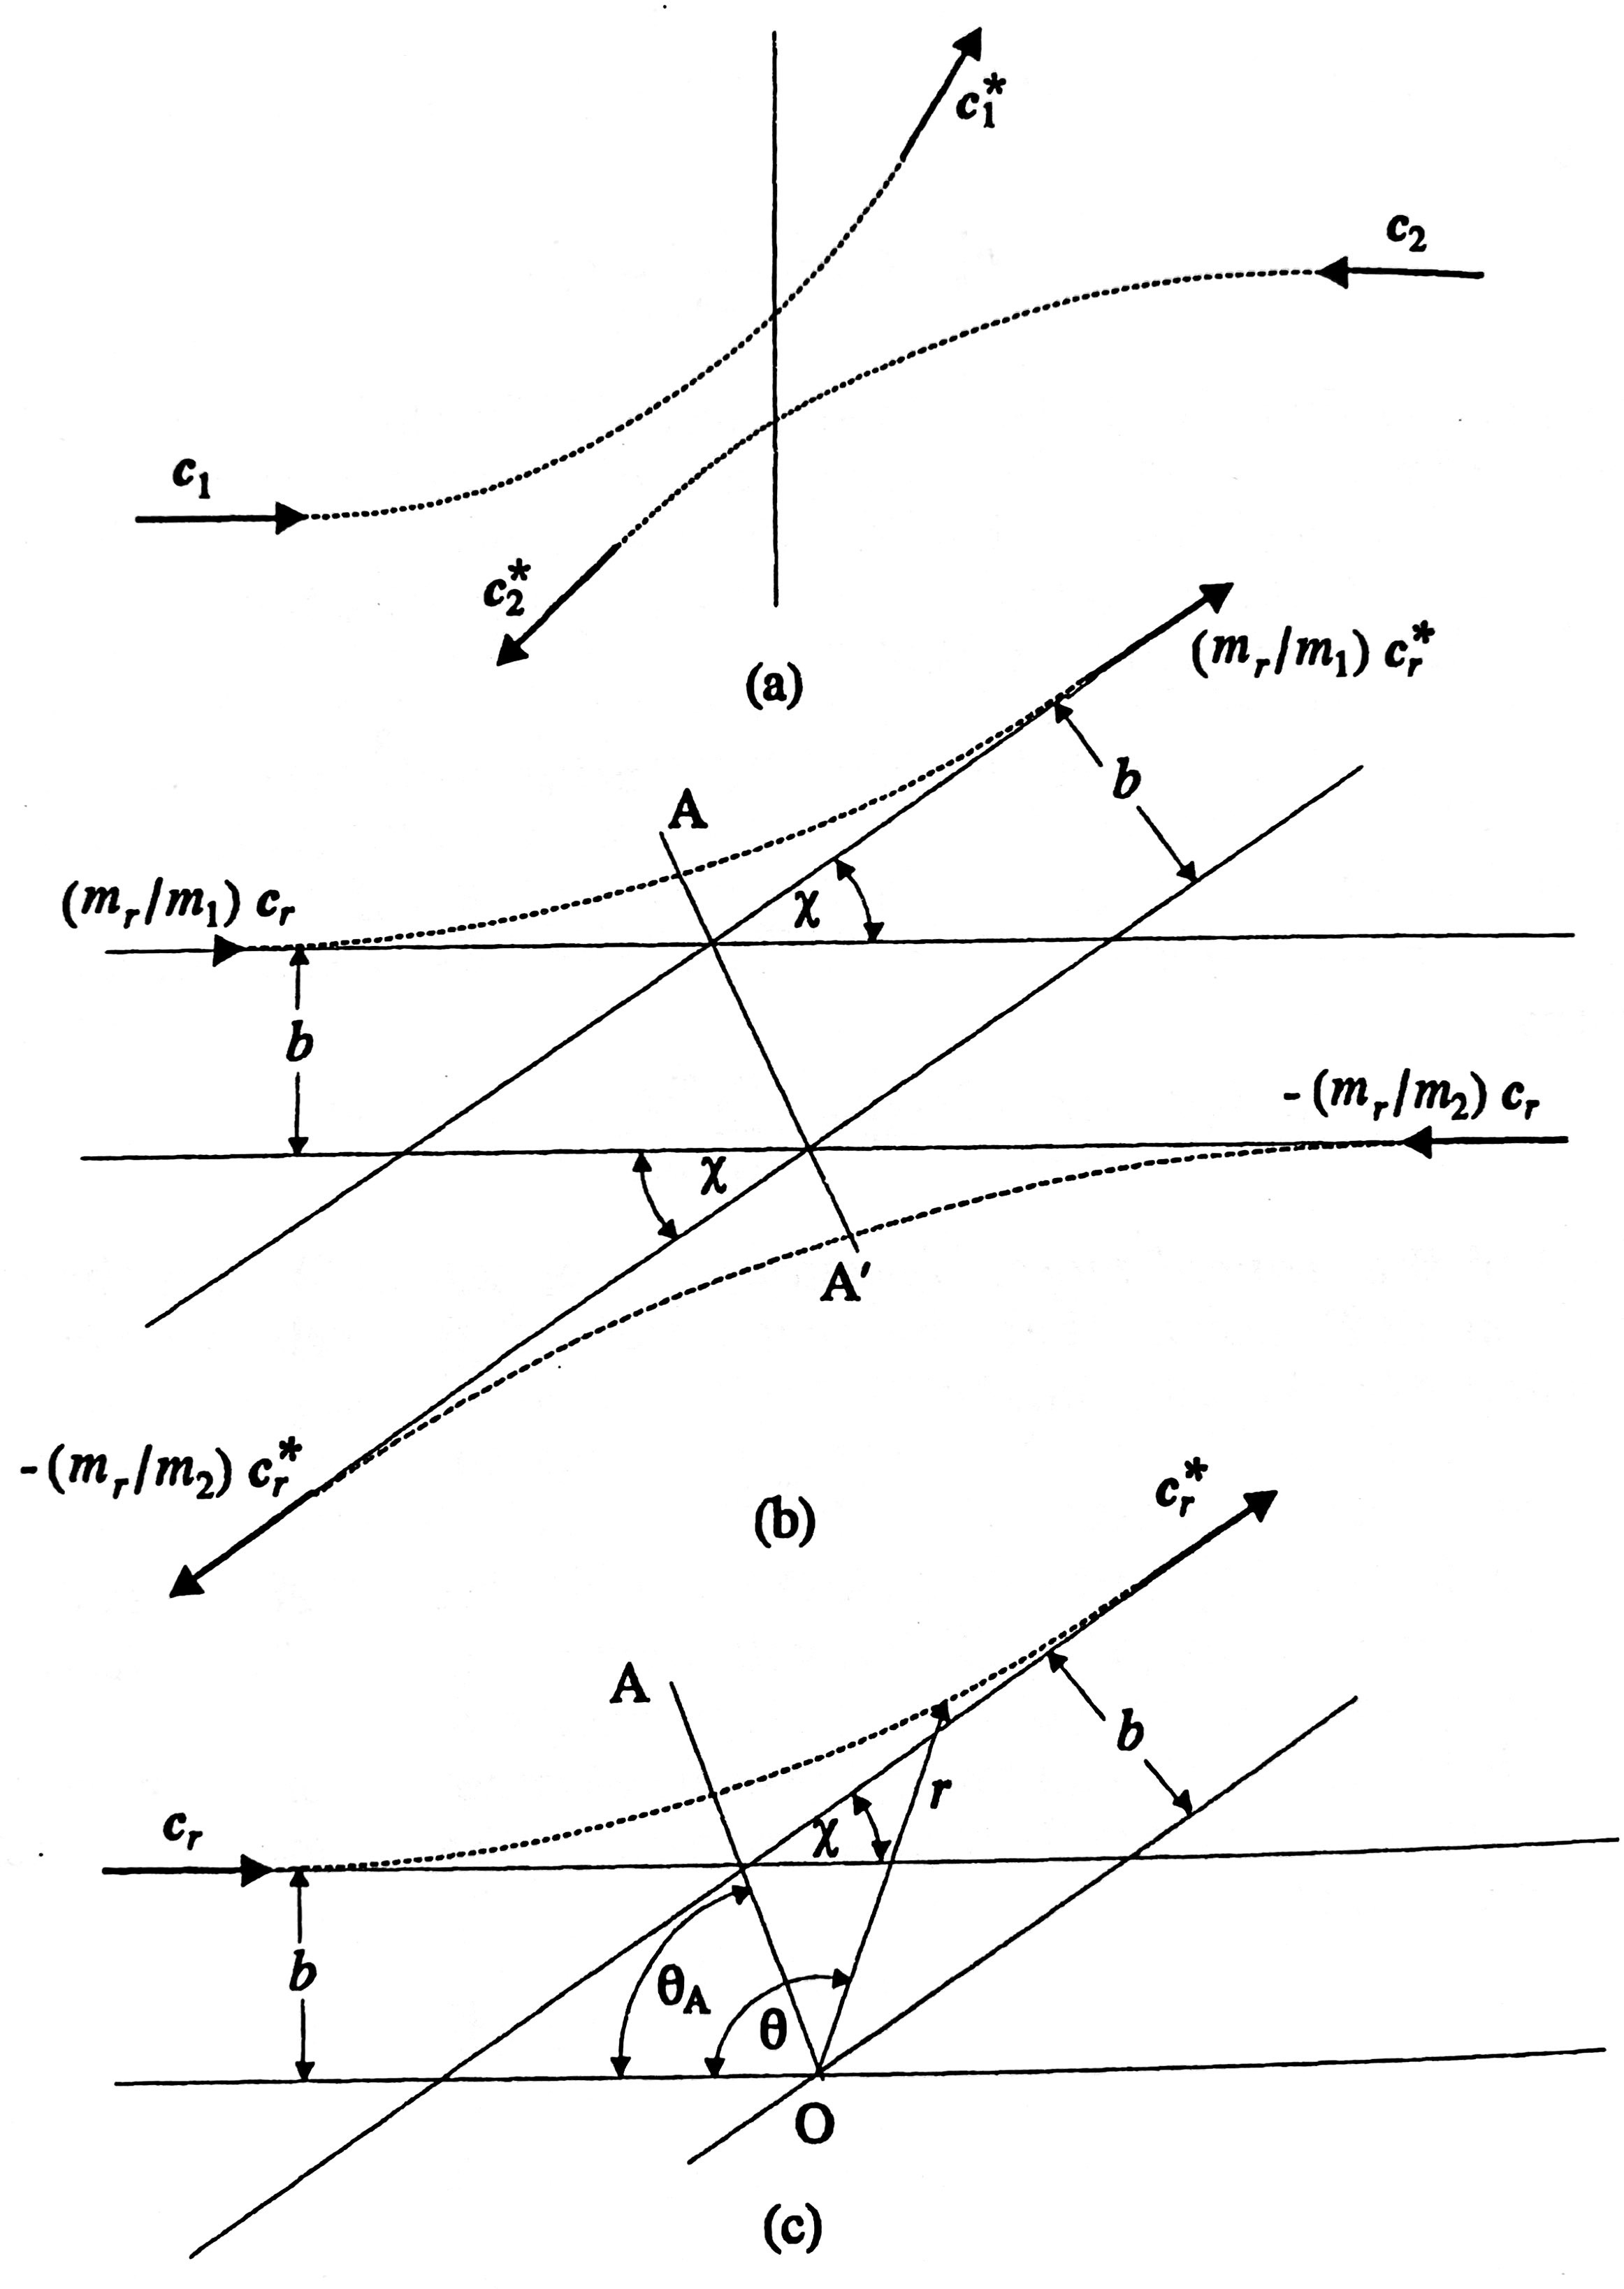
\includegraphics[width=10cm]{fig/dsmc/bird1.jpg}
    \caption{2体衝突の表現 : (a) 基準となる実験系,(b) 基準の重心座標系での2体衝突,(c) 換算質量粒子と固定散乱中心の相互作用~\cite{bird1994molecular}.}
    \label{fig:bird1}
\end{figure}

\subsection{衝撃パラメータと衝突断面積}
2つの分子の速度を分離して,弾性衝突を表すためには2つの衝撃パラメータが必要となる.
1つ目は,重心座標系での乱れていない軌道の最も近いアプローチ$b$の距離で,
2つ目は,Collision planeとReference planeの角度$\varepsilon$である.
ただし,分子の衝突前および衝突後の軌道は,同じ平面である.

パラメータ$b$および$\varepsilon$は,特定の偏向角$\chi$を与える.
パラメータ$b$と$\varepsilon$に対応する微分断面積$\sigma \mathrm{d}\Omega$は,
\begin{equation}
    \sigma \mathrm{d}\Omega = b{\rm d}b\mathrm{d}\varepsilon,
\end{equation}
であり,$\mathrm{d}\Omega$はベクトル$c_r^*$方向の微小立体角である.
図~\ref{fig:bird2}より,
\begin{equation}
    \mathrm{d}\Omega = \sin \chi\mathrm{d}\chi\mathrm{d}\varepsilon,
\end{equation}
従って,
\begin{equation}
    \sigma = \dfrac{b}{|\sin\chi|}\dfrac{\mathrm{d}b}{\mathrm{d}\chi}.
\end{equation}
また,全衝突断面積$\sigma_T$は次式で表される.
\begin{equation}
    \sigma_T = \int_0^{4\pi}\sigma\mathrm{d}\Omega = 2\pi\int_0^\pi \sigma\sin\chi\mathrm{d}\chi.
\end{equation}
さらに粘性係数の断面積$\sigma_\mu$は次式のようになる.
\begin{equation}
    \sigma_\mu = \int_0^{4\pi}\left( \sin^2 \chi \right)\sigma\mathrm{d}\Omega 
    = 2\pi\int_0^\pi \left(\sin^3 \chi\right)\sigma\sin \chi\mathrm{d}\chi.
\end{equation}
衝突前の速度方向に垂直となる衝突後の速度成分は$c_r\sin \chi$である.
この積分は,粘性係数を算出するために,Chapman–Enskog理論~\cite{bird1994molecular}で用いられる.

拡散断面積とも呼ばれる運動量輸送断面積は,
\begin{equation}
    \sigma_M = \int_0^{4\pi}\left(1 - \cos \chi\right)\sigma\mathrm{d}\Omega 
    = 2\pi\int_0^\pi \left(1-\cos \chi\right)\sin \chi\mathrm{d}\chi.
\end{equation}
粘性係数の断面積と同様にして,
衝突前の速度方向に垂直となる衝突後の速度成分は$c_r\left(1 - \cos \chi\right)$である.
この積分は,拡散係数を算出するために,Chapman–Enskog理論~\cite{bird1994molecular}で用いられる.

\begin{figure}
    \centering
    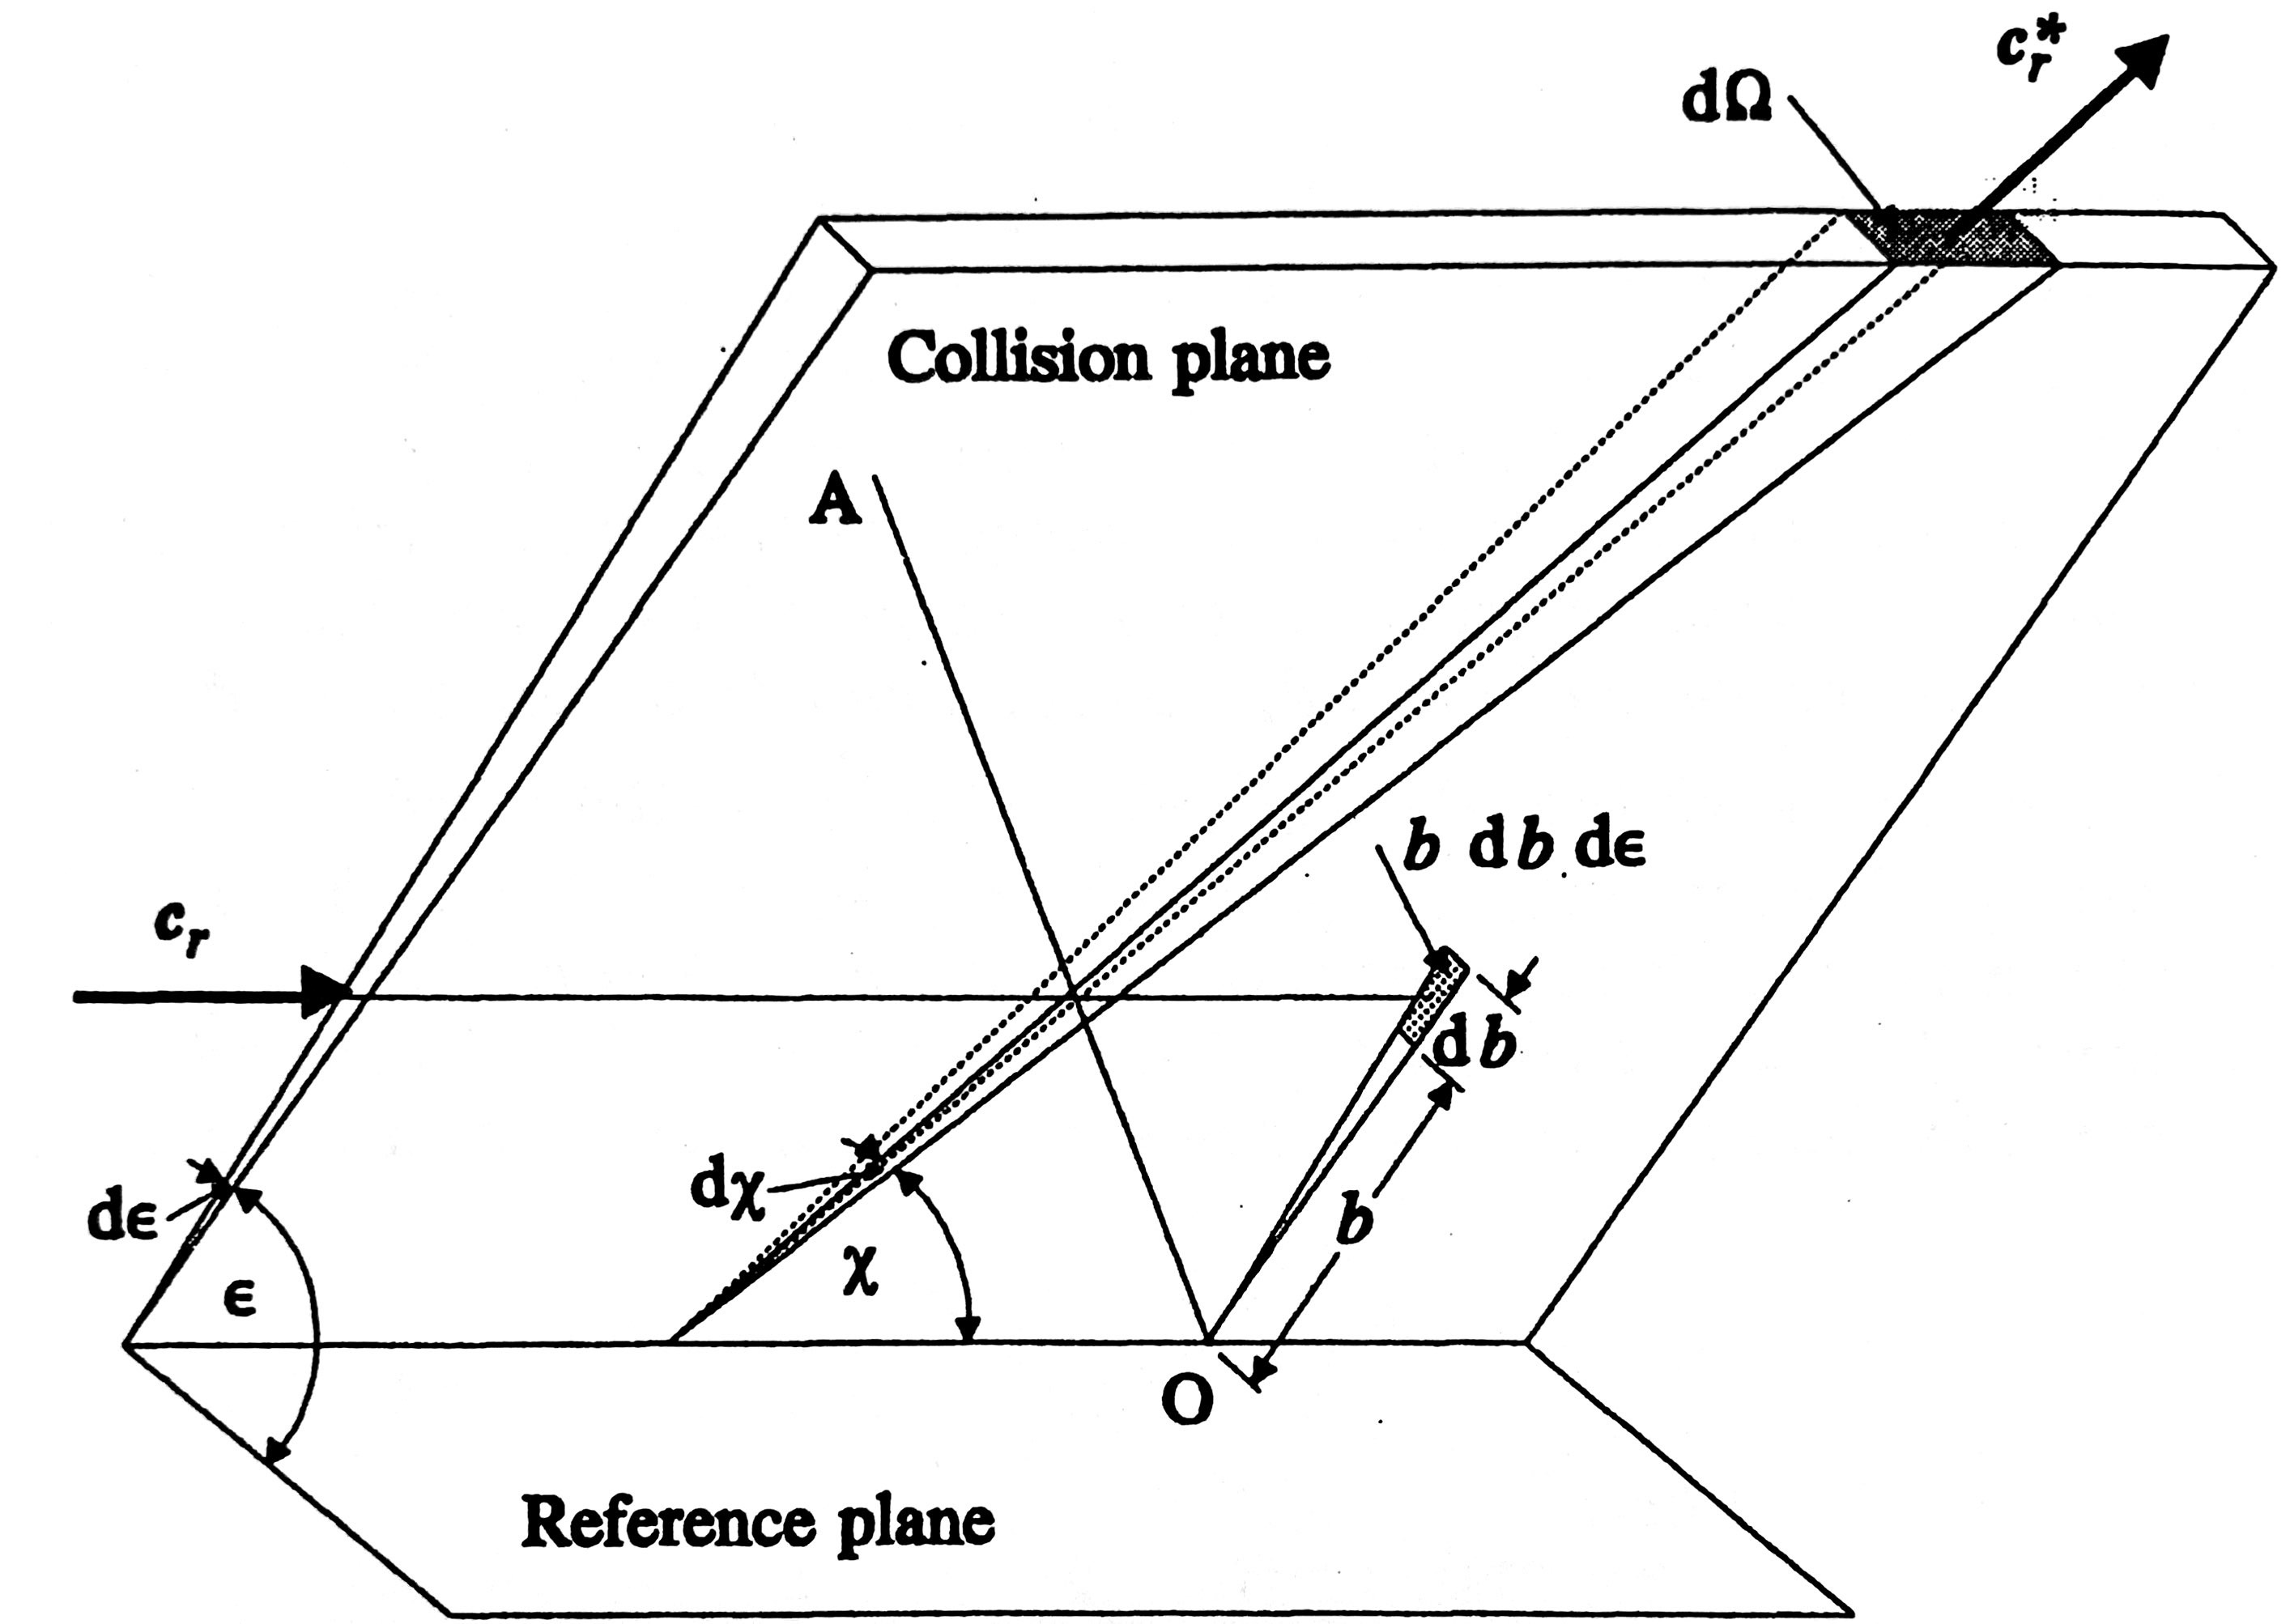
\includegraphics[width=10cm]{fig/dsmc/bird2.jpg}
    \caption{衝突パラメータ~\cite{bird1994molecular}.}
    \label{fig:bird2}
\end{figure}

\subsection{Variable Soft Sphere モデル}
DSMC法における衝突は,物理モデルと計算効率の双方を考慮した分子モデルを選択する必要がある.
近年のDSMC法で一般に用いられる分子モデルとして,
KouraとMatsumoto~\cite{koura1991variable}により提唱されたVariable Soft Sphere (VSS) モデルがある.
VSSモデルでは接触の瞬間に無限の反発力を持ち,
それ以外の場合は力を及ぼさない弾性球として分子を扱う.
このモデルでは分子の直径$d$と相対速度$c_r$の関係は以下のようになる.
\begin{equation}
    d \propto c_r^{(1/2)-\omega}.
\end{equation}
ただし,$\omega$はモデルパラメータである.
また,偏向角は衝突パラメータ$b$を用いて次式のようになる.
\begin{equation}
    \chi = 2\cos^{-1}\left(\dfrac{b}{a}\right)^{1/a}.
\end{equation}
ここで,$a$はVSSモデルの散乱パラメータで,VSSモデルでの全衝突断面積は
$\sigma_T  = \pi d^2$で与えられる.
これによりVSSモデルでの粘性係数が求められて,
\begin{equation}
    \mu=\dfrac{5}{16} \frac{(\alpha+1)(\alpha+2) \sqrt{\pi m k}\left(\frac{4 k}{m}\right)^{\xi} T^{\frac{1}{2}+\xi}}{\alpha \Gamma(4-\xi) \sigma_{T, \mathrm{ref}} c_{r, \mathrm{ref}}^{2 \xi}},
\end{equation}
となる.

VSSモデルは単純でかつ,
平衡~\cite{gallis2004molecular}および非平衡~\cite{gallis2011investigation}両方の条件下で単原子分子の輸送特性を正確に予測できるため,DSMC法で良く用いられる.
さらに,より現実的であるが計算コストがより高いLennard–JonesポテンシャルやMorseポテンシャルと比較すると計算効率がより高いという特徴もあり,
本研究ではVSSモデルを使用する.

\begin{table}[H]
    \centering
    \caption{本研究で用いるVSSモデルのパラメータ}
    \begin{tabular}{c|cccc}
    \hline\hline
        化学種 & $d$~[m] & $\omega$~[$-$] & $T_\mathrm{ref}$~[K] & $\alpha$~[$-$] \\ \hline
        \ce{O2} & \num{3.96d-10} & 0.77 & 273.15 & 1.4 \\
        \ce{N2} & \num{4.07d-10} & 0.77 & 273.15 & 1.6 \\
        \ce{O} & \num{3.00d-10} & 0.77 & 273.15 & 1.0 \\
        \ce{N} & \num{3.00d-10} & 0.77 & 273.15 & 1.0 \\
        \ce{NO} & \num{4.00d-10} & 0.77 & 273.15 & 1.0 \\
        \hline\hline
    \end{tabular}
    \label{tab:vss}
\end{table}

\subsection{内部エネルギー}
多原子分子においては内部エネルギーモードが存在するため,
多原子分子の衝突を記述するには並進および内部のエネルギー状態との緩和断面積が必要である.
ただし,全ての断面が分かっている場合でも,多数の遷移があるためこの方法は複雑化する.

多原子分子を効率よく計算する方法としては,単原子分子のモデルに多原子分子の機能を追加するという手法がある.
従って,VSSモデルに内部エネルギーモードと並進および内部エネルギー交換を行う方法を追加することで,多原子分子へと拡張する.
内部エネルギーモードは自由度$\xi$によって特徴付けられる.

DSMC法においては,現象論的なLarsen–Borgnakke(GLB)モデルがエネルギー交換に用いられる.
このGLBモデルでの非弾性衝突後の内部エネルギーは,
全エネルギーの平衡分布からサンプリングし以下のように割り当てられる.
\begin{align}
f\left(\dfrac{E_{t r}}{E_{c}}\right) &= \dfrac{\Gamma[5 / 2-\omega+\zeta]}{\Gamma[5 / 2-\omega] \Gamma[\zeta]}\left(\dfrac{E_{t r}}{E_{c}}\right)^{3 / 2-\omega}\left(1-\dfrac{E_{t r}}{E_{c}}\right)^{\zeta-1} \\
f\left(\dfrac{E_{i}}{E_{c}}\right) &= \dfrac{\Gamma[5 / 2-\omega+\zeta]}{\Gamma[5 / 2-\omega] \Gamma[\zeta]}\left(1-\dfrac{E_{i}}{E_{c}}\right)^{3 / 2-\omega}\left(\dfrac{E_{i}}{E_{c}}\right)^{\zeta-1}
\end{align}
ただし,$E_{tr}$は並進エネルギー,$E_i$は内部エネルギー,$E_c = E_{tr} + E_i$は衝突分子ペアの
全エネルギー,$\gamma$はガンマ関数である.
衝突モデルは,$\omega$を介して平衡分布となるため,
平衡分布を実際に衝突している分子の分布から区別している~\cite{bird1994molecular}.

回転エネルギーと異なり,
並進エネルギーよりも広い間隔のエネルギー状態を持つため,振動モードは完全には励起されない.
従って,エネルギー状態を連続的に記述するよりも離散的な記述が必要である.
2原子分子の振動モードの離散的なエネルギー状態は,それぞれがポテンシャルおよび運動エネルギーから影響され,
調和振動子モデルおよび非調和振動子モデルを使用して記述される.

\subsection{化学反応モデル}
空気の中性粒子そのイオンから成るNASA Air–11混合気体の化学反応は,
Parkのメカニズムによって説明されている~\cite{park1993review,park2001chemical}.
このメカニズムには一酸化窒素の解離反応が考慮されており,
流星周りにおける一酸化窒素の存在は過去に研究がなされている~\cite{menees1976nitric,park1978odd,silber2018nitric}.

本研究における化学反応はBird~\cite{bird1994molecular}によるTotal Collision Energy (TCE) 法を用いる.
TCEモデルでは既知の反応係数に基づいて反応確率を定義する.

%\subsection{速度分布関数}
%期待中の分子すべてが同じ速度で運動しているわけではないため,分子運動を取り扱い祭にはどの速度をもった分子がどれくらい存在するかを表す速度分布関数が必要になる.
%位置を$\bm{x}$とすると,ある位置での分子数密度は$n(\bm{x})$と書ける.
%その位置を含む微小検査体積$\mathrm{d}v = \mathrm{d}x\mathrm{d}y\mathrm{d}z$の中にある分子の数は$n(\bm{x})\mathrm{d}v$になる.
%分子の速度$c$の直交座標成分を$c_1,\ c_2,\ c_3$として,それぞれを座標軸とした速度空間を考え,
%ある速度空間でのベクトル$\bm{c}$の先端に体積$\mathrm{d}c = \mathrm{d}c_1\mathrm{d}c_2\mathrm{d}c_3$の直方体を考える.
%この中にある分子の数は分子速度関数$f$を用いて$fn\mathrm{d}c$と書くことができ,$c\sim c+\mathrm{d}c$の速度を持つ分子の数を表す.$f$は速度空間の市によって変わるため$c$の関数であり,
%速度空間すべての分子数を加えると全体の分子数に等しいという以下に示す条件を満たす必要がある.
%\begin{equation}
%    \int^\infty_{-\infty}\!\int^\infty_{-\infty}\!\int^\infty_{-\infty}
%    fn\mathrm{d}c = n
%\end{equation}
%
%非定常流れでは$n$は時間$t$の関数でもあるため,それに伴って$f$も位置と時間の関数になる.

\subsection{SPARTAカーネル}
DSMC法を実行可能なオープンソースコードとして,
MONACO~\cite{padilla2010comparison}やDAC~\cite{padilla2010comparison},dsmcFoam(+)~\cite{scanlon2010open,white2018dsmcfoam+,raeisi2019numerical}などがあるが,
本研究におけるDSMC法の計算コードにはSPARTAカーネル~\cite{spartaWWW,bariselli2020aerothermodynamic,plimpton2019direct}を用いた.
SPARTAはGPLライセンスのオープンソースソフトウェアとして配布され,
単列計算または,MPIライブラリを用いた領域分割による並列計算が可能である.
DSMC法への理解と入力ファイルの記述が必要になる.

入力ファイルは以下のような4つの手順によって記述される.
\begin{enumerate}
    \item 初期化
    \item 問題定義
    \item 条件設定
    \item シミュレーションの開始
\end{enumerate}
3番目および4番目の手順は計算が収束するまで反復することができる.

\subsubsection{1. 初期化}
ここでは,シミュレーションに必要なパラメータの設定を行う.
ここで設定するパラメータは単位系 (CGS単位系またはSI単位系),
乱数に用いるシード値,
計算領域の次元 (2次元または3次元) が含まれる.

\subsubsection{2. 問題定義}
ここでは,シミュレーションの開始に必要となる全てのパラメータを設定する.
計算領域となるボックスの大きさ,
計算領域境界におけるサンプル粒子の振る舞い,
格子数の設定,
計算領域内部における固体表面の設置,
粒子の分子組成と初期状態の設定などが含まれる.

\subsubsection{3. 条件設定}
初期化および問題定義の次は入力ファイルでの条件設定を行う.
ここでは,出力方法や出力する物理量,
衝突モデル,化学モデル,並列計算での動的負荷分散,
境界条件,固体表面での反射モデルの選択などを定義する.
この部分はシミュレーション結果の品質に大きく関わり,重要である.
さらにこの部分では,
固体表面の特性計算,時間刻み幅,サンプリング間隔も具体的に定義する.
サンプリング間隔の設定が適切に行われないと結果の品質が著しく低下し,
出力結果の書き込み頻度は計算時間に大きく影響するため慎重に指定する必要がある.
